%%%%%%%%%%%%%%%%%%%%%%%%%%%%%%%%%%%%%%%%%
% baposter Landscape Poster
% LaTeX Template
% Version 1.0 (11/06/13)
%
% baposter Class Created by:
% Brian Amberg (baposter@brian-amberg.de)
%
% This template has been downloaded from:
% http://www.LaTeXTemplates.com
%
% License:
% CC BY-NC-SA 3.0 (http://creativecommons.org/licenses/by-nc-sa/3.0/)
%
%%%%%%%%%%%%%%%%%%%%%%%%%%%%%%%%%%%%%%%%%

%----------------------------------------------------------------------------------------
%	PACKAGES AND OTHER DOCUMENT CONFIGURATIONS
%----------------------------------------------------------------------------------------

\documentclass[portrait,a0paper,fontscale=0.285]{baposter} % Adjust the font scale/size here

\usepackage{graphicx} % Required for including images
\graphicspath{{figures/}} % Directory in which figures are stored

\usepackage{amsmath} % For typesetting math
\usepackage{amssymb} % Adds new symbols to be used in math mode
\usepackage{tabularx}

\usepackage{booktabs} % Top and bottom rules for tables
\usepackage{enumitem} % Used to reduce itemize/enumerate spacing
\usepackage{palatino} % Use the Palatino font
\usepackage[font=small,labelfont=bf]{caption} % Required for specifying captions to tables and figures
\usepackage{grffile} % can use other graphics extensions (e.g. doesn't error for example.0.1.png)
\usepackage{caption}
\usepackage{cite}

\usepackage{multicol} % Required for multiple columns
\usepackage{url} % For references which have website URLs
\setlength{\columnsep}{1.5em} % Slightly increase the space between columns
\setlength{\columnseprule}{0mm} % No horizontal rule between columns

\usepackage{tikz} % Required for flow chart
\usetikzlibrary{shapes,arrows} % Tikz libraries required for the flow chart in the template

\usepackage{array}
\newcolumntype{P}[1]{>{\centering\arraybackslash\vspace{-2mm}}p{#1}} % P-alignment in tables ensures both vertical and horizontal centered.

\newcommand{\compresslist}{ % Define a command to reduce spacing within itemize/enumerate environments, this is used right after \begin{itemize} or \begin{enumerate}
\setlength{\itemsep}{0pt}
\setlength{\parskip}{0pt}
\setlength{\parsep}{0pt}
}

\setlist[itemize]{leftmargin=*}

%\definecolor{lightblue}{rgb}{0.145,0.6666,1} % Defines the color used for content box headers
\definecolor{lightblue}{rgb}{1,0.3333,0.3333} %not very 'light blue'

\begin{document}

\begin{poster}
{
headerborder=closed, % Adds a border around the header of content boxes
colspacing=1em, % Column spacing
bgColorOne=white, % Background color for the gradient on the left side of the poster
bgColorTwo=white, % Background color for the gradient on the right side of the poster
borderColor=lightblue, % Border color
headerColorOne=black, % Background color for the header in the content boxes (left side)
headerColorTwo=lightblue, % Background color for the header in the content boxes (right side)
headerFontColor=white, % Text color for the header text in the content boxes
boxColorOne=white, % Background color of the content boxes
textborder=roundedleft, % Format of the border around content boxes, can be: none, bars, coils, triangles, rectangle, rounded, roundedsmall, roundedright or faded
eyecatcher=true, % Set to false for ignoring the left logo in the title and move the title left
headerheight=0.1\textheight, % Height of the header
headershape=roundedright, % Specify the rounded corner in the content box headers, can be: rectangle, small-rounded, roundedright, roundedleft or rounded
headerfont=\Large\bf\textsc, % Large, bold and sans serif font in the headers of content boxes
%textfont={\setlength{\parindent}{1.5em}}, % Uncomment for paragraph indentation
linewidth=2pt % Width of the border lines around content boxes
}
%----------------------------------------------------------------------------------------
%	TITLE SECTION 
%----------------------------------------------------------------------------------------
%
{
\includegraphics[height=3em]{Figures/IITlogo.png}} % First university/lab logo on the left
{\bf\huge{\hspace{-1.5in}Hybrid Methods for Simulation \\ \hspace{-1.5in}of Muon Ionization Cooling Channels}\vspace{0.1em}} % Poster title
{{ \large{\hspace{-1.5in}J. Kunz, P. Snopok$^1$ \hspace{12pt} Illinois Institute of Technology \\\hspace{-1.5in}M. Berz \hspace{12pt}Michigan State University \\\hspace{-1.5in}$^1$ also at Fermi National Accelerator Laboratory \vspace{-0.4em}}}}
{
\includegraphics[height=6em]{Figures/MAPlogo.png}} % Second university/lab logo on the right

%----------------------------------------------------------------------------------------
%	MICE Layout
%----------------------------------------------------------------------------------------

\headerbox{Muon Ionization Cooling Experiment (MICE) Layout}{name=mice,column=0,row=0,span=2}{
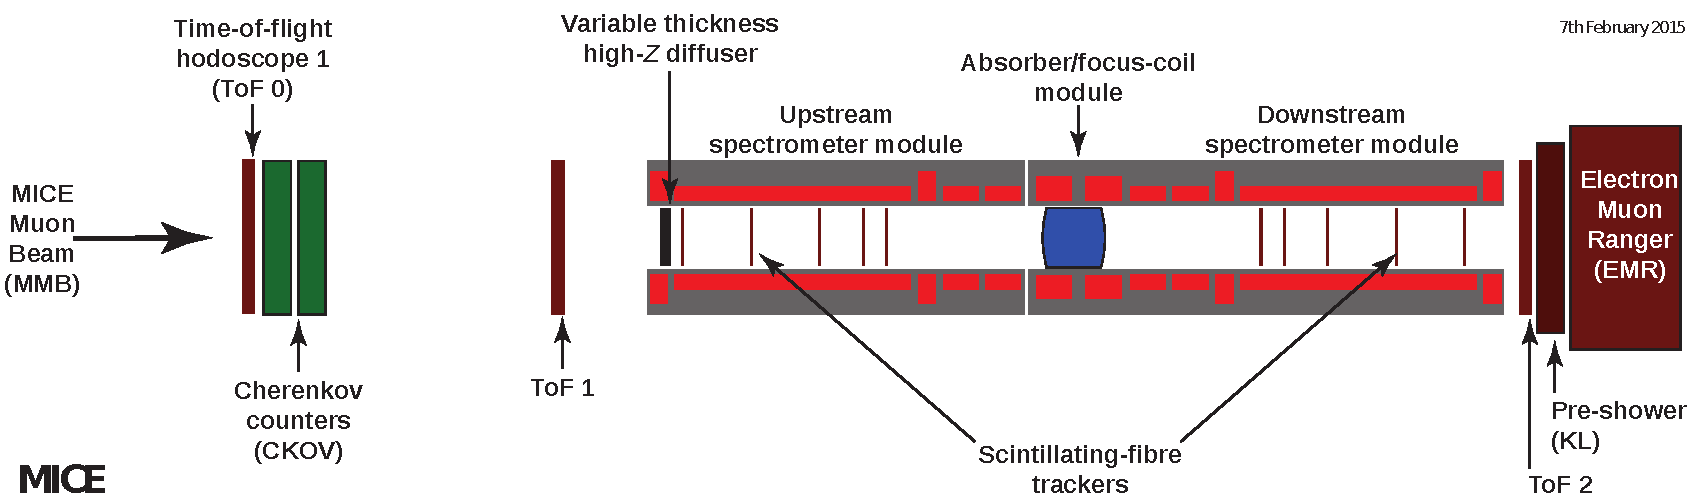
\includegraphics[width=0.9\textwidth]{Figures/mice}
}

%----------------------------------------------------------------------------------------
%	Absorbers
%----------------------------------------------------------------------------------------

\headerbox{Ionization cooling}{name=absorbers,column=0,row=1,below=mice}
{
\begin{itemize}
\item Muons are tertiary production particles ($ p \rightarrow \pi \rightarrow \mu $). As a result, the muon beam phase space volume is very large.
\item Muons must be focused and accelerated within the muon lifetime (2.2~$\mu$s in the rest frame). The only cooling technique that is fast enough is ionization cooling.
\item Muons traverse an absorber, momentum is lost both in the longitudinal and transverse directions due to ionization. The energy is then restored in the longitudinal direction only, leading to an overall reduction in the transverse beam size.
\item To achieve cooling in the longitudinal direction, emittance exchange is used, typically involving wedge-shaped absorbers.
\item For some applications such as a high-energy high-luminosity muon collider, cooling has to be very aggressive: 6D emittance reduction over six orders of magnitude to reach design goals.
\item Recently, an arbitrary-order transfer map simulation code COSY Infinity \cite{cosy} has been outfitted with new hybrid transfer map--Monter Carlo tools for matter-dominated muon ionization cooling lattices. \item Excellent agreement has been achieved between COSY, G4Beamline \cite{g4bl}, and ICOOL \cite{icool} for pencil beams of $p=$ (100, 200, 300, 400) MeV/$c$ through liquid hydrogen absorbers of lengths $L =$ (1, 10, 100) mm.
\item Agreement has been shown with the \mbox{MuScat} results \cite{muscat}. An example of a collimated beam of 172~MeV/$c$ muons passing through 109~mm of liquid hydrogen is shown below.
\end{itemize}
\begin{center}
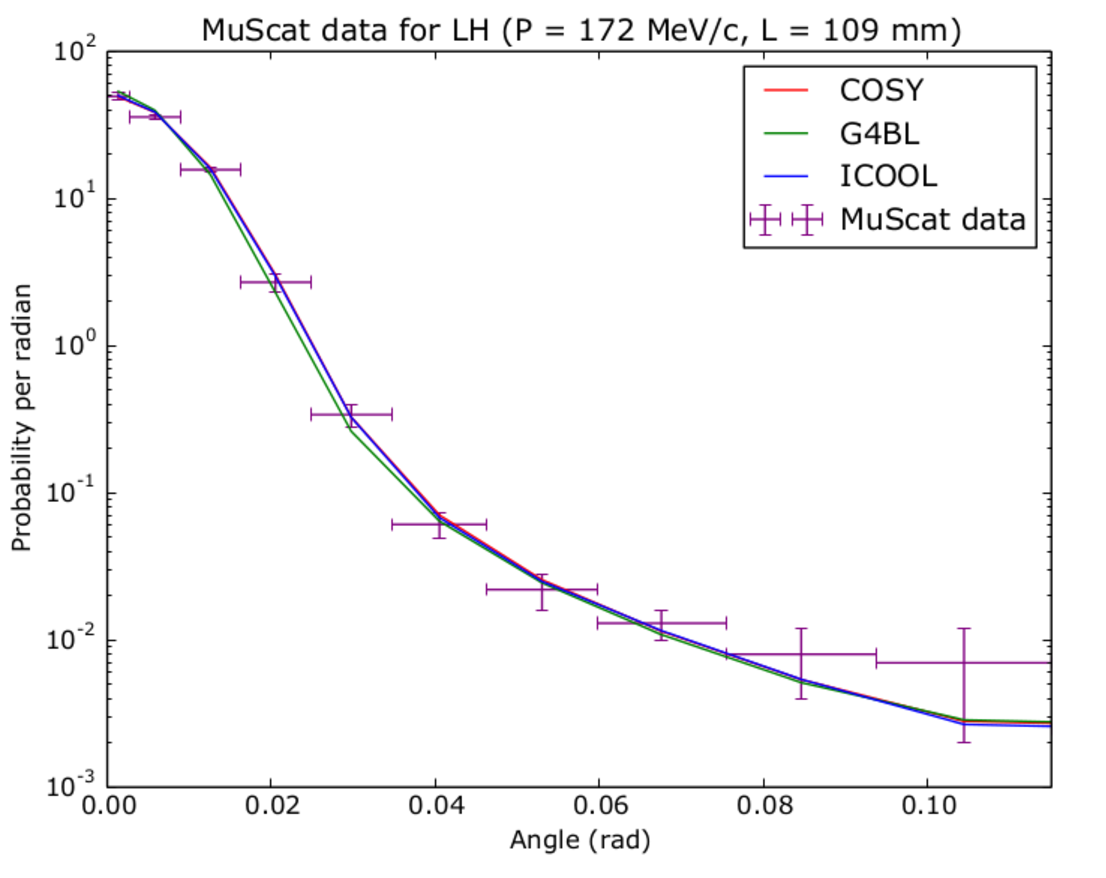
\includegraphics[width=\textwidth]{Figures/Figure2poster}
\end{center}
}

%----------------------------------------------------------------------------------------
%	Stochastic Processes
%----------------------------------------------------------------------------------------
\headerbox{Stochastic Processes}{name=stochastic,column=1,row=1,below=mice}
{
\begin{itemize}
\item The stochastic processes of interest are energy straggling and multiple scattering.
\item Straggling follows Landau theory.
\item The derivation of the scattering function is done separately for small and large angles: Gaussian for small angles and Rutherford-like for large angles.
\item Both algorithms with time-of-flight and multiple scattering offset corrections were implemented in COSY and applied to MICE~\cite{mice}.
\end{itemize}
}


%----------------------------------------------------------------------------------------
%	MICE Cell
%----------------------------------------------------------------------------------------

\headerbox{MICE cell}{name=micecell,column=1,row=1,below=stochastic}
{
\begin{itemize}
\item MICE simulations use the Step IV geometry shown in the figure above.
\item Piecewise transfer maps of order 5 were used to represent the complex magnetic field accurately.
\item The initial distribution was Gaussian with the following parameters: $\sigma_{x,y}=32$~mm, $\sigma_{p_x,p_y}=20$~MeV$/c$, $\sigma_{p_z}=30$~MeV$/c$.
\item The absorber was a cylindrical lithium hydride block of 65 mm or a 350 mm volume of liquid hydrogen.
\item The beam was propagated from the center of the upstream spectrometer module to the center of the downstream spectrometer module (see figure above).
\item Coil parameters are summarized in the table below. Inner radius is 258 mm for all coils.
\end{itemize}
\begin{footnotesize}
\begin{tabularx}{\columnwidth}{ccccc}
\toprule
Name & $z$ & Length & Outer & Current \\
 & position & & radius & density \\
 & mm & mm & mm & A/mm$^2$  \\
\midrule
	End2 & $\mp$3200 &111  &326 &$\pm$126 \\
	Center&$\mp$2450 &1314 &280 &$\pm$148 \\
	End1 & $\mp$1700 & 111 & 319 & $\pm$133 \\
	Match2 & $\mp$1300 & 199 & 289 & $\pm$132 \\
	Match1 & $\mp$861 & 201 & 304 & $\pm133$ \\
	Focus & $\mp$202 & 213 & 362 & $\pm$104 \\ 
\bottomrule
\end{tabularx}
\end{footnotesize}
}

%----------------------------------------------------------------------------------------
%	References
%----------------------------------------------------------------------------------------

\headerbox{References}{name=references,column=1,row=1,below=micecell,span=2}
{
\renewcommand{\section}[2]{}% Gets rid of header
\begin{footnotesize}
%\bibliography{bib}{}
%\bibliographystyle{plain}
\begin{thebibliography}{9}
\bibitem{cosy}
K. Makino, M. Berz, COSY INFINITY Version 9, \emph{Nuclear Instruments and Methods} \textbf{A558} (2005) 346-350,\\ see also \url{http://www.cosyinfinity.org}
\bibitem{icool} 
R. C. Fernow \emph{et al.,} ICOOL Simulation Code, \url{http://www.cap.bnl.gov/ICOOL/}

\bibitem{g4bl}
T. Roberts, G4Beamline, \url{http://www.muonsinternal.com/muons3/G4Beamline}

\bibitem{muscat}
D. Attwood \emph{et al.} (2006), The scattering of muons in low-Z materials, NIM B251, p. 41

\bibitem{mice}
A. Blondel \emph{et al.,} (2003), Tech. rep., MICE-NOTE-21, \url{http://mice.iit.edu/mnp/MICE0021.pdf} 

\end{thebibliography}
\end{footnotesize}
}

%----------------------------------------------------------------------------------------
% 	MICE Results
%----------------------------------------------------------------------------------------

\headerbox{MICE Results}{name=miceResults,column=2,row=0,bottomaligned=micecell}
{
The results of the MICE simulation with 350~mm of liquid hydrogen:
\begin{center}
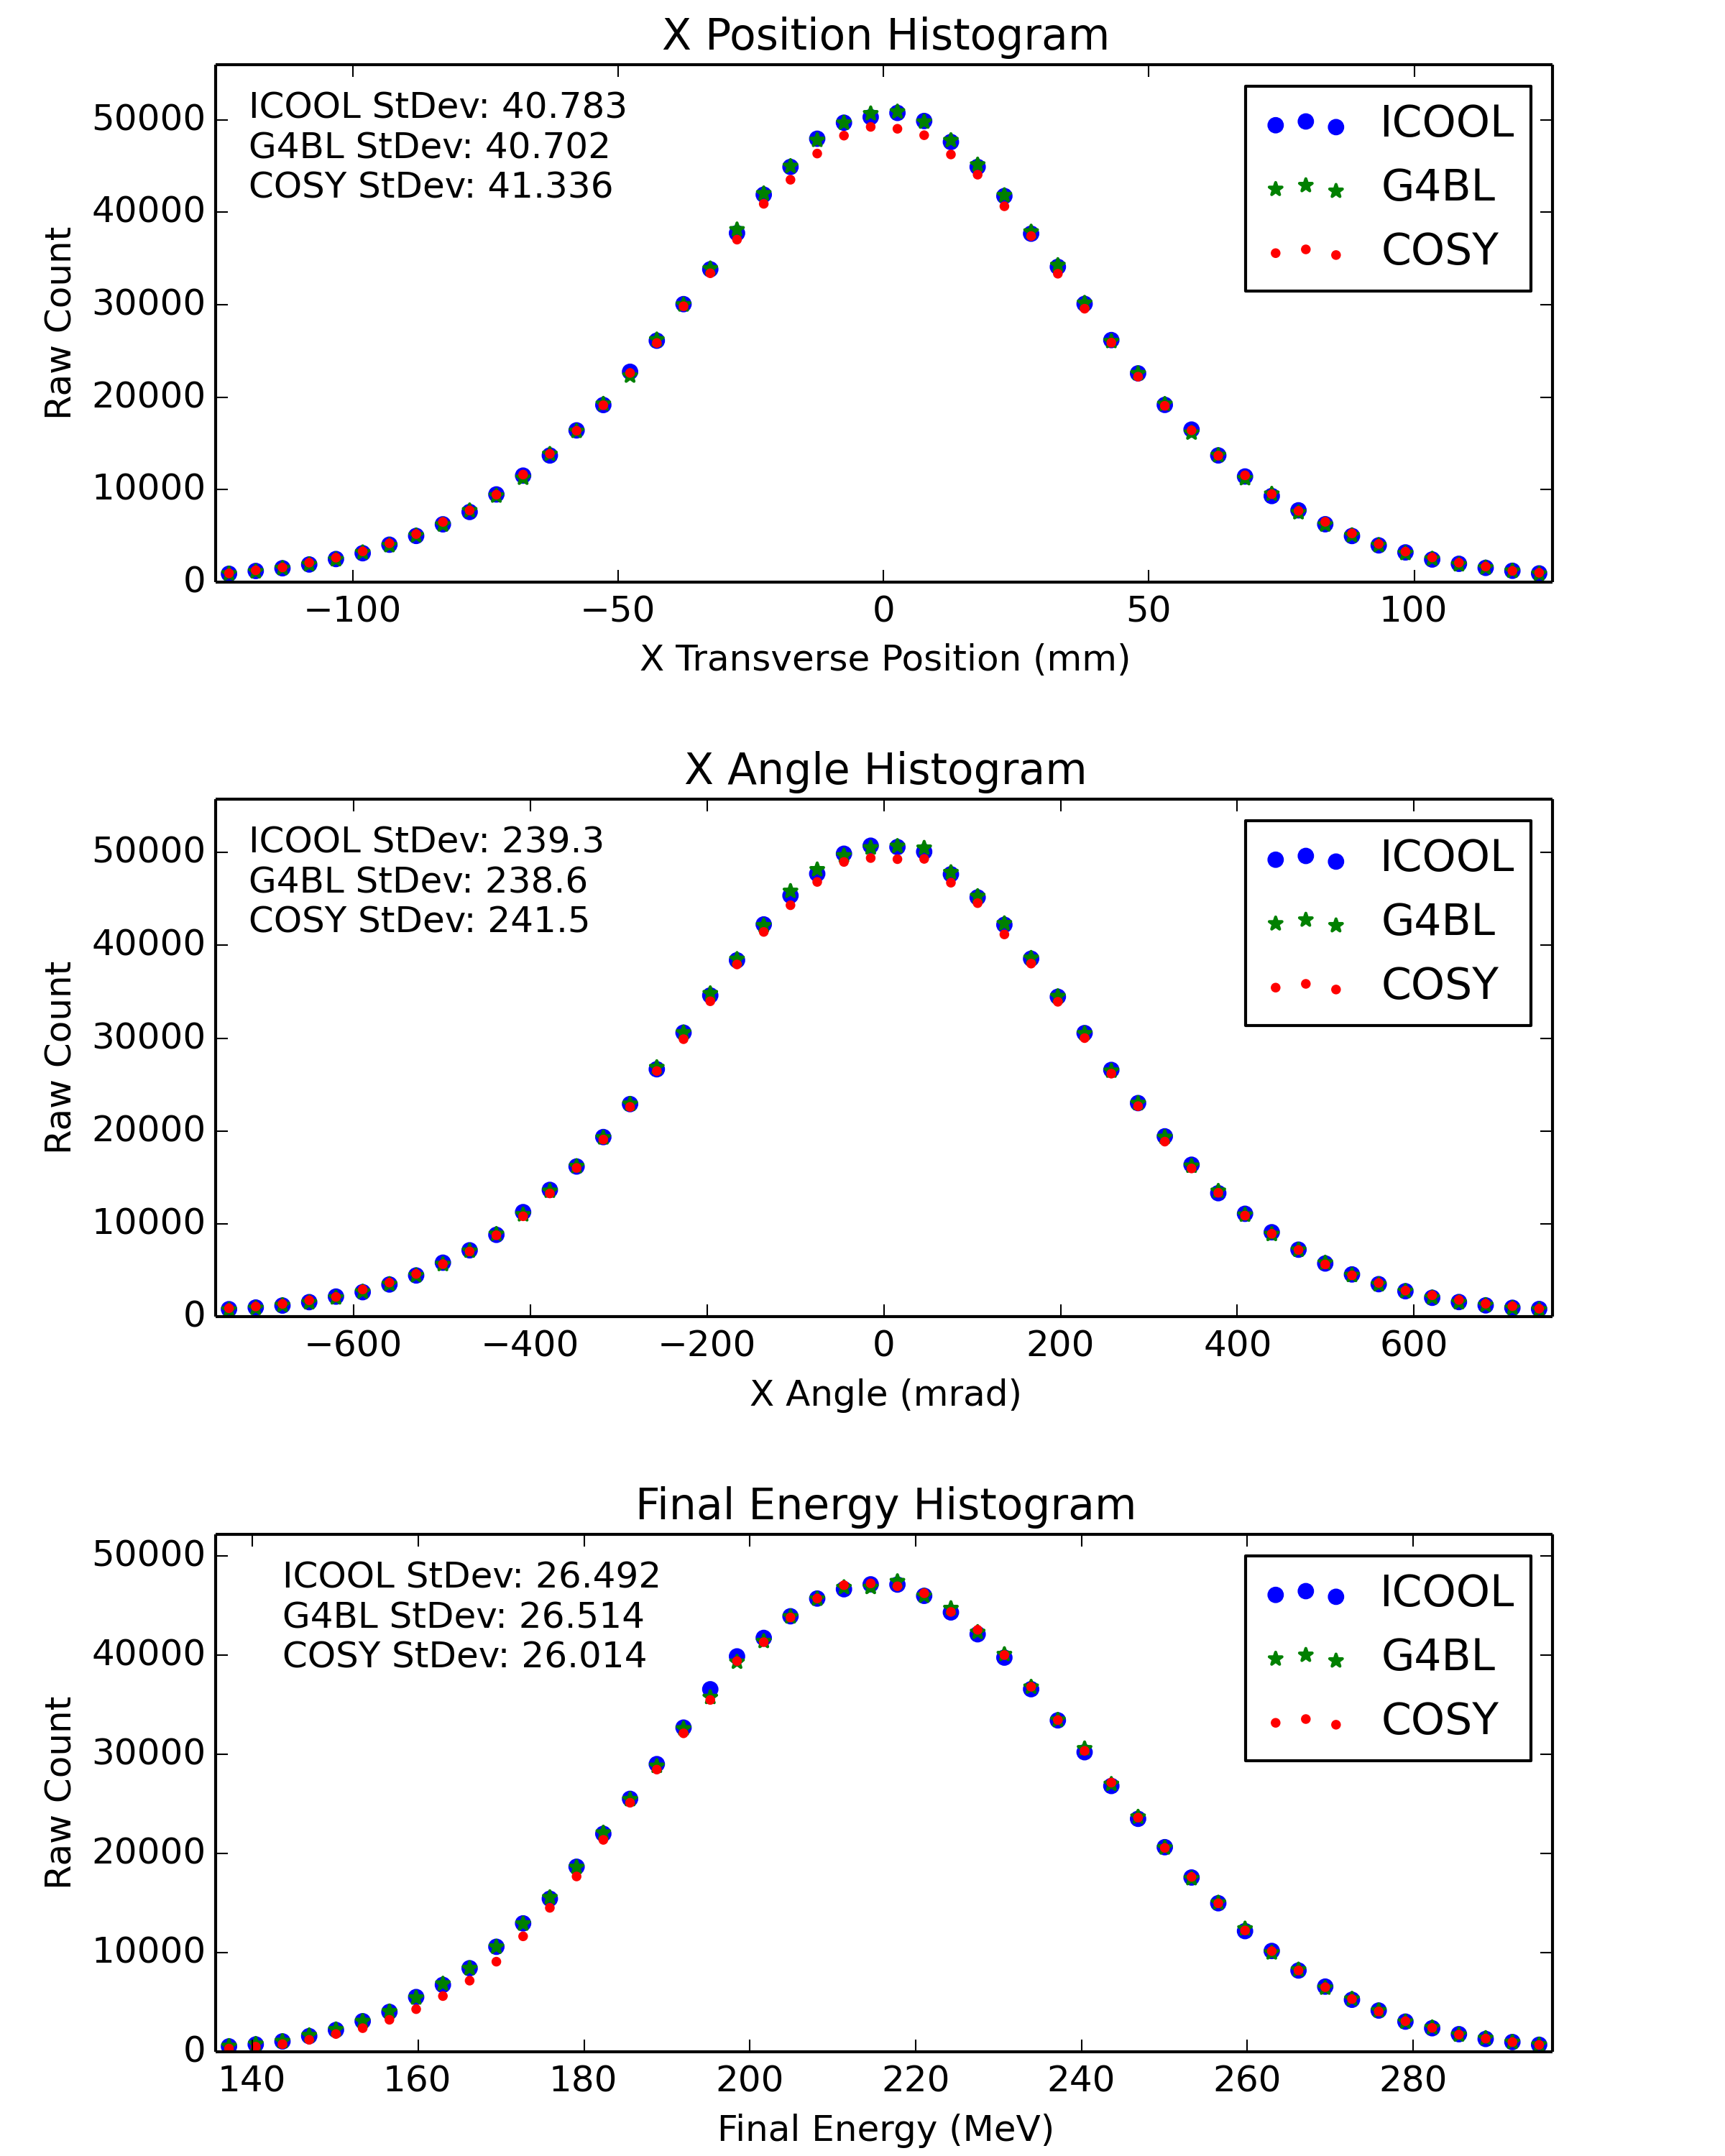
\includegraphics[width=\textwidth]{Figures/MICE_LH}
\end{center}

Simulation with 65~mm of lithium hydride:

\begin{center}
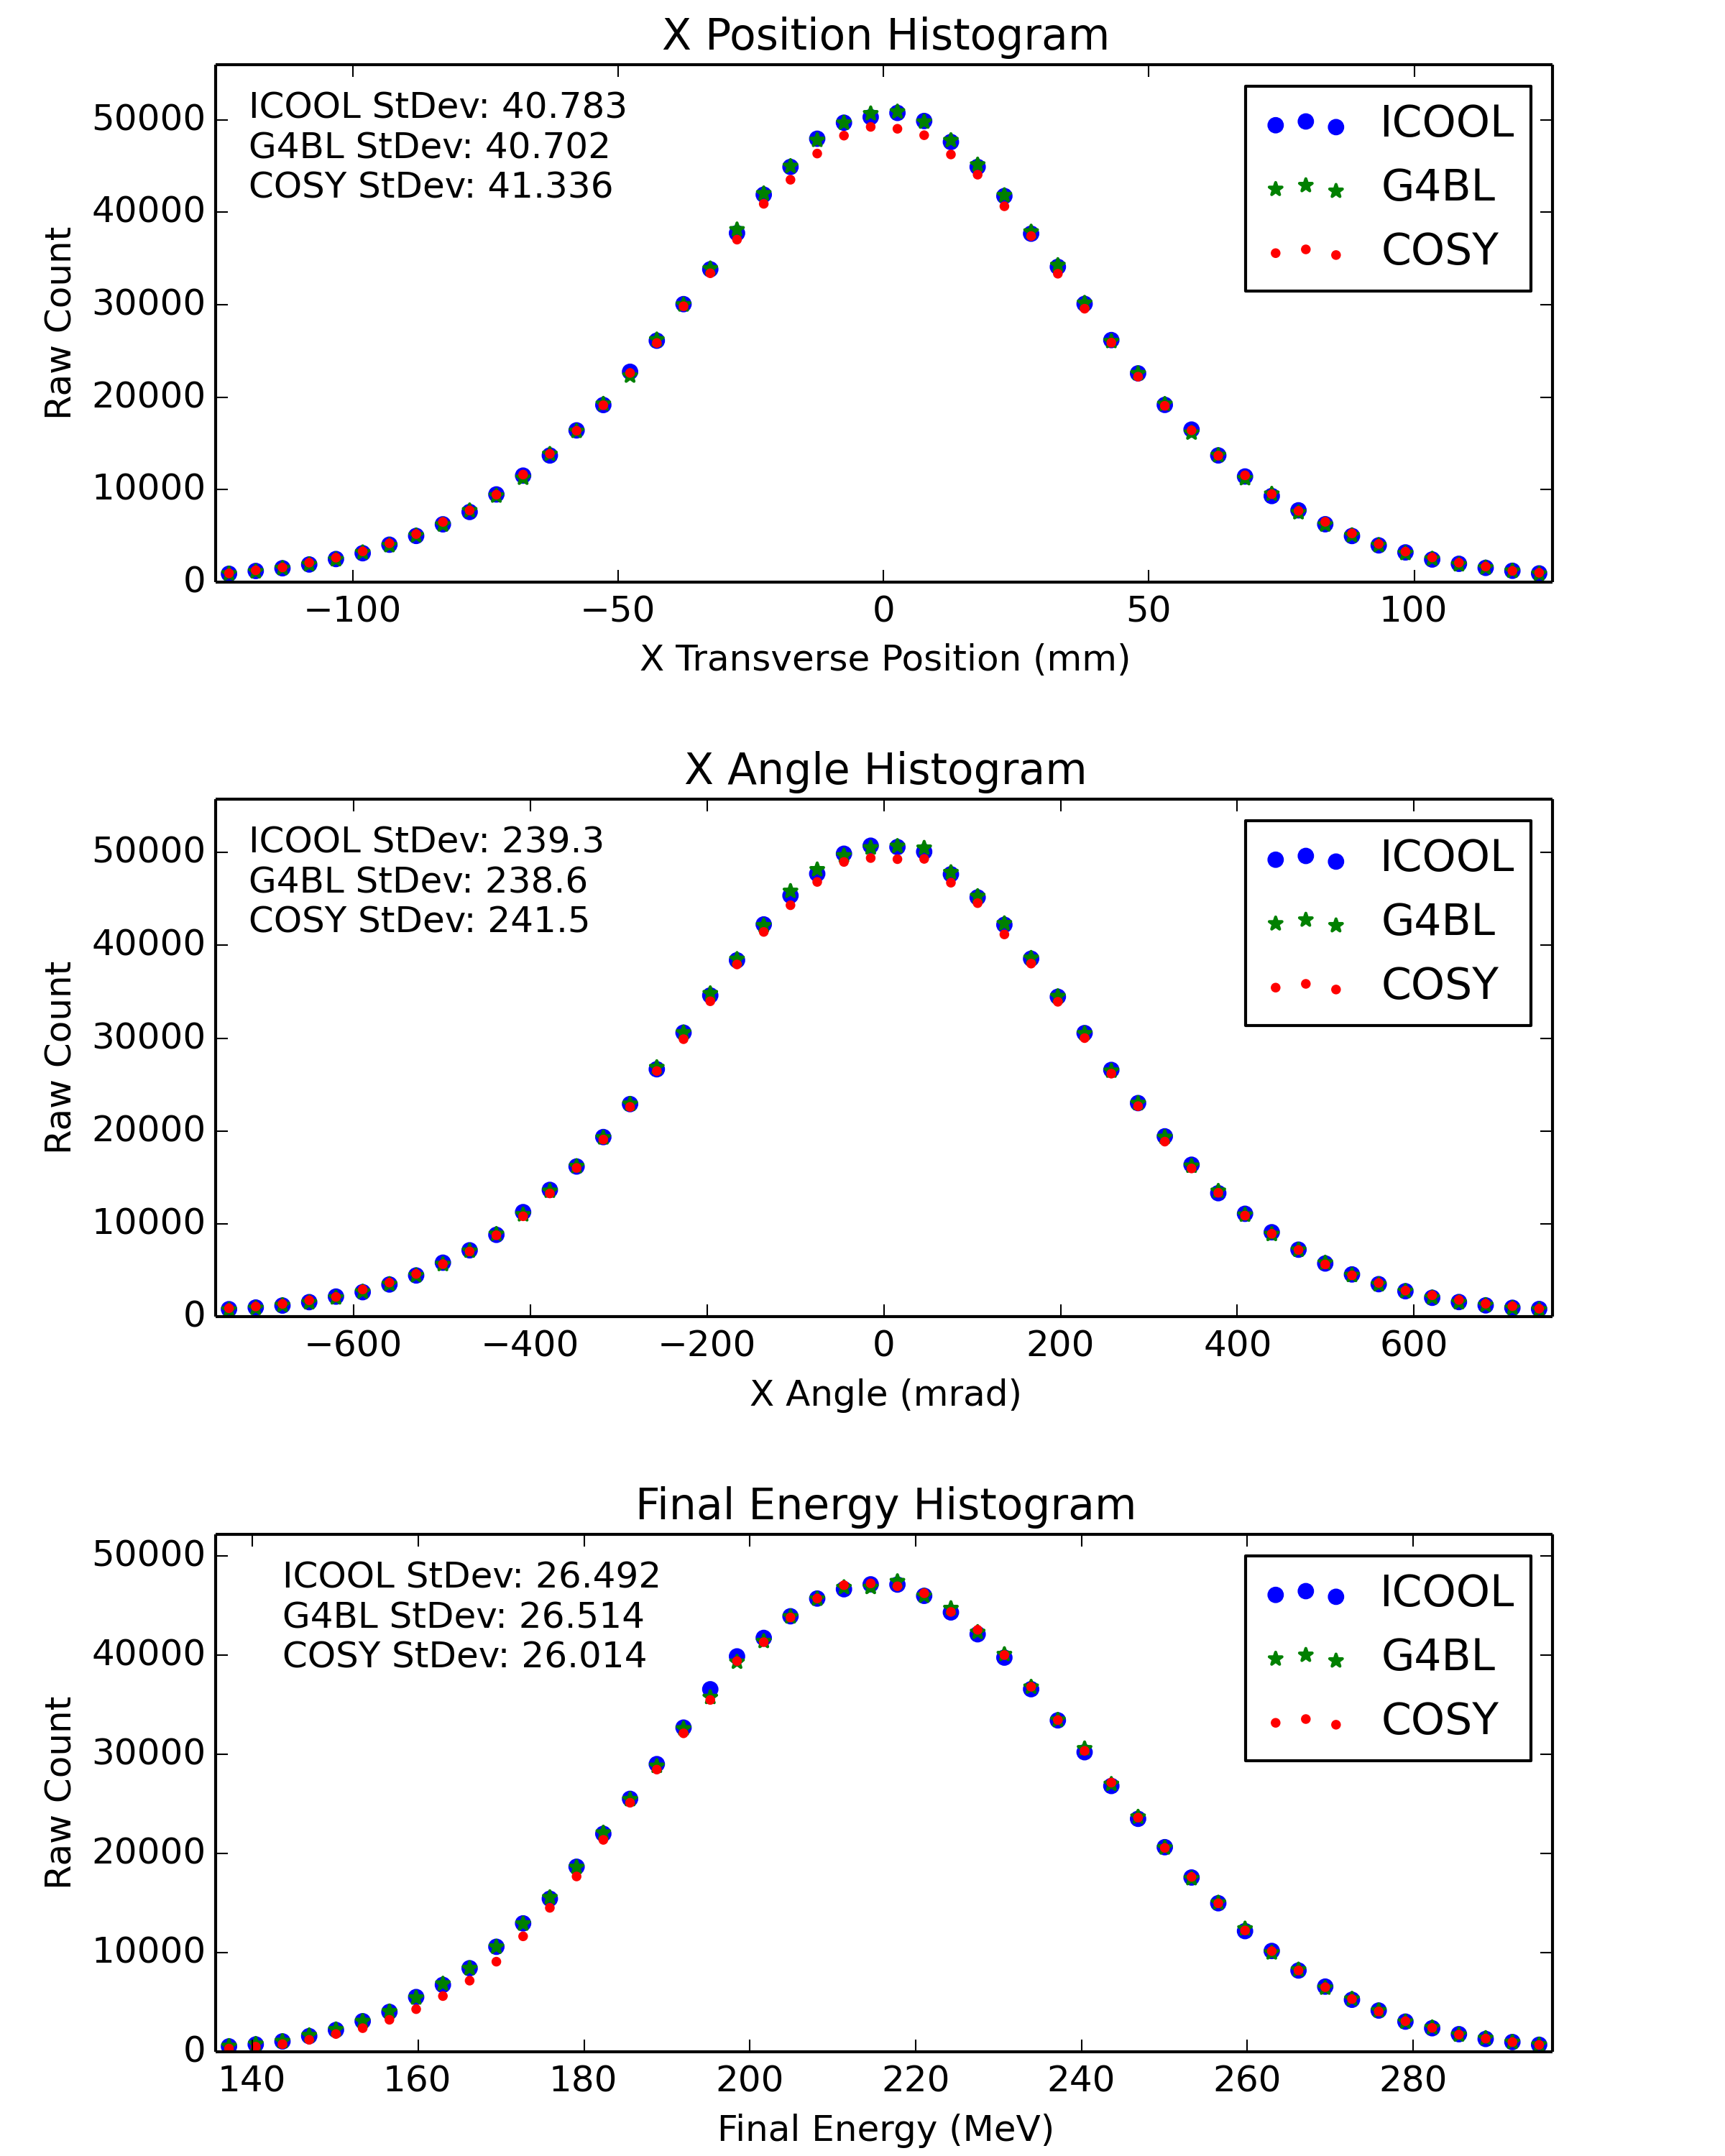
\includegraphics[width=\textwidth]{Figures/MICE_LH}
\end{center}

Computational times for liquid hydrogen are summarized below. The new hybrid approach in COSY is about twice as fast as G4Beamline and about three times as fast as ICOOL.
%\iffalse
%\begin{table}
%\caption*{\textbf{Run Times (in seconds) for MICE Step IV Simulation}}
\begin{center}
\begin{small}
\begin{tabularx}{\columnwidth}{ccccc}
%\vspace{-40pt}\\ 
\toprule
Number of particles: & $10^6$ & $10^5$ & $10^4$ & $10^3$\\
\midrule
COSY: & 367 & 31 & 6 & 4\\
G4BL (coils): & 3973 & 392 & 40 & 6\\
G4BL (field map): & 662 & 75 & 15 & 9\\
ICOOL (field map): & 1091 & 117 & 19 & 9\\
\bottomrule
\end{tabularx}
\end{small}
\end{center}
%\caption[Run times for MICE Step IV simulation.]{Run times for MICE Step IV simulation for liquid hydrogen. Note that the G4Beamline initialization time was not added to the run time values. G4BL (coils) represents the simulation in G4Beamline when the \texttt{coil} parameter was used. G4BL (field map) represents the simulation when G4Beamline (like ICOOL) read the field map from a file.}
%\label{tbl:mice_times}
%\end{table}
%\fi
}

\end{poster}

\end{document}